\documentclass[10pt,letterpaper,bibliography=totoc]{scrartcl}

\usepackage[letterpaper,margin=1.2in]{geometry}
\usepackage{helvet}
\usepackage[utf8]{inputenc}
\usepackage{graphicx}
\usepackage[hyphens]{url}
\usepackage{hyperref}
\usepackage[all]{hypcap} 
\usepackage{xcolor}
\usepackage{listings}
\usepackage[T1]{fontenc}
\usepackage{verbatim}
\usepackage[parfill]{parskip}

\lstset{
    basicstyle=\scriptsize,
    numbers=left,
    numberstyle=\scriptsize,
    stepnumber=1,
    numbersep=5pt,
    showspaces=false,
    showstringspaces=false,
    showtabs=false,
    frame=shadowbox,
    tabsize=4,
    captionpos=b,
    breaklines=true,
    breakatwhitespace=false,
    keywordstyle=\color{blue!70},
    commentstyle=\color{red!50!green!50!blue!50},
    rulesepcolor=\color{red!20!green!20!blue!20},
    numberbychapter=false,
    stringstyle=\ttfamily
}

\setcounter{tocdepth}{2}

\hypersetup{
    colorlinks=true,
    breaklinks=true,
    urlcolor=blue,
    linkcolor=black
}

\begin{document}

\author{Orkun Krand}
\title{Assignment 5}
\subtitle{Fall 2017\\ CS834 Introduction to Information Retrieval\\ Dr. Michael Nelson}
\maketitle
\newpage

\section{Question 10.5}
\subsection {Question}
Find a community-based question answering site on the Web and ask two questions, one that is low-quality and one that is high-quality. Describe the answer quality of each question.

\subsection{Answer}
I decided to use \href{www.quora.com}{Quora} to answer this question. My high quality question was: ``How does a clutch work?'' This is a high quality question because it is asking for serious information on how a car part operates. As expected, the answers were serious as well with some providing images to support the answer. There were no jokes or funny remarks. Because Quora classifies questions into topics, nobody thought the question was about women's purses or the 1990s rock band. 

\begin{figure}[h!]
\centering
\label{fig:clutch}
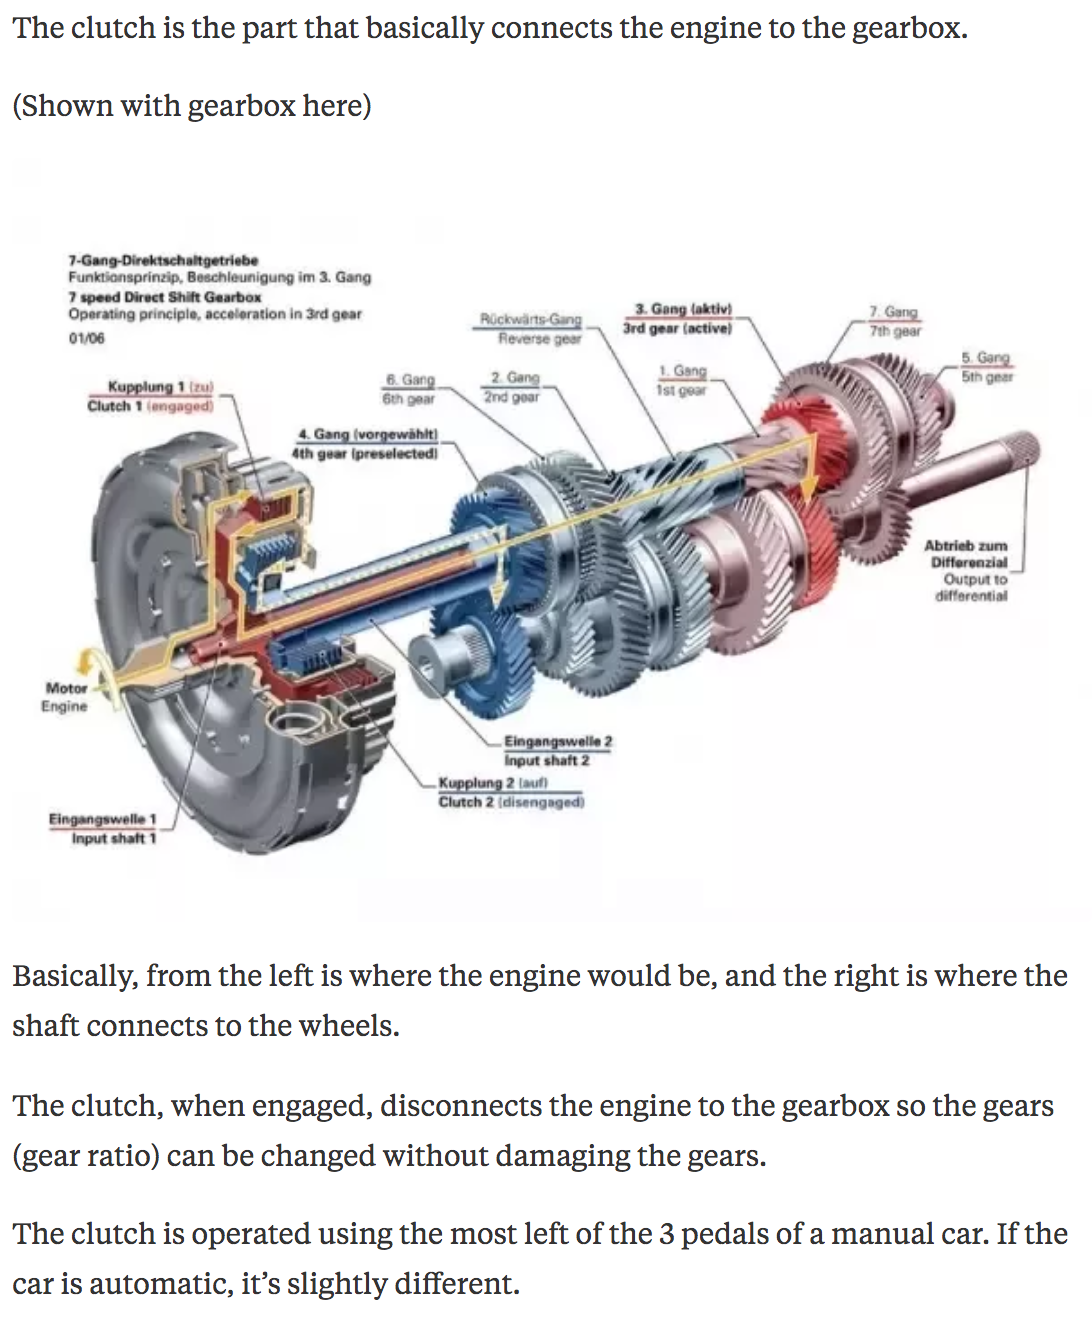
\includegraphics[scale=.5]{clutch.png}
\caption{How does a clutch work}
\end{figure}

My low quality question was: ``Why do motorcycle riders always feel compelled to wave at other motorcycle riders in passing, or when coming to a stop light?'' The reason the words ``feel compelled'' is used is to show that this question isn't really looking for a valid reason but it is more of a fun question. It's not a technical question that has one answer, it also isn't a universal case but the United States or North America isn't mentioned in the question. The purpose of the question was to ask about the origin of the motorcyclist wave, but because of the way it was worded and the way the wave actually works (or doesn't), it can't be considered a high quality question.

\begin{figure}[h!]
\centering
\label{fig:low_quality}
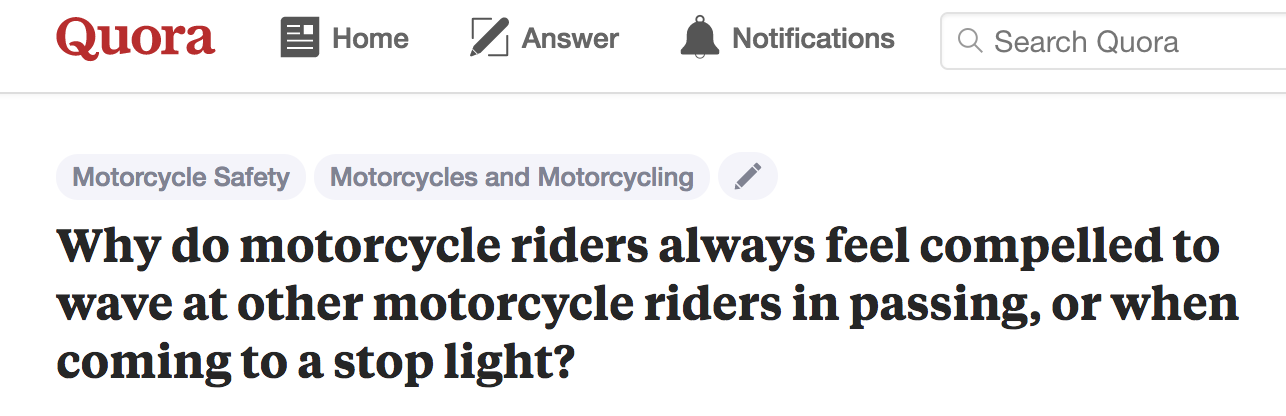
\includegraphics[scale=.5]{low_quality.png}
\caption{Low quality question}
\end{figure}

The answers posted were mostly entertaining with one person listing reasons why people who own a certain brand of bike won't wave back. I can safely say that I did not learn anything from the answers to this question.

\begin{figure}[h!]
\centering
\label{fig:reasons_wave}
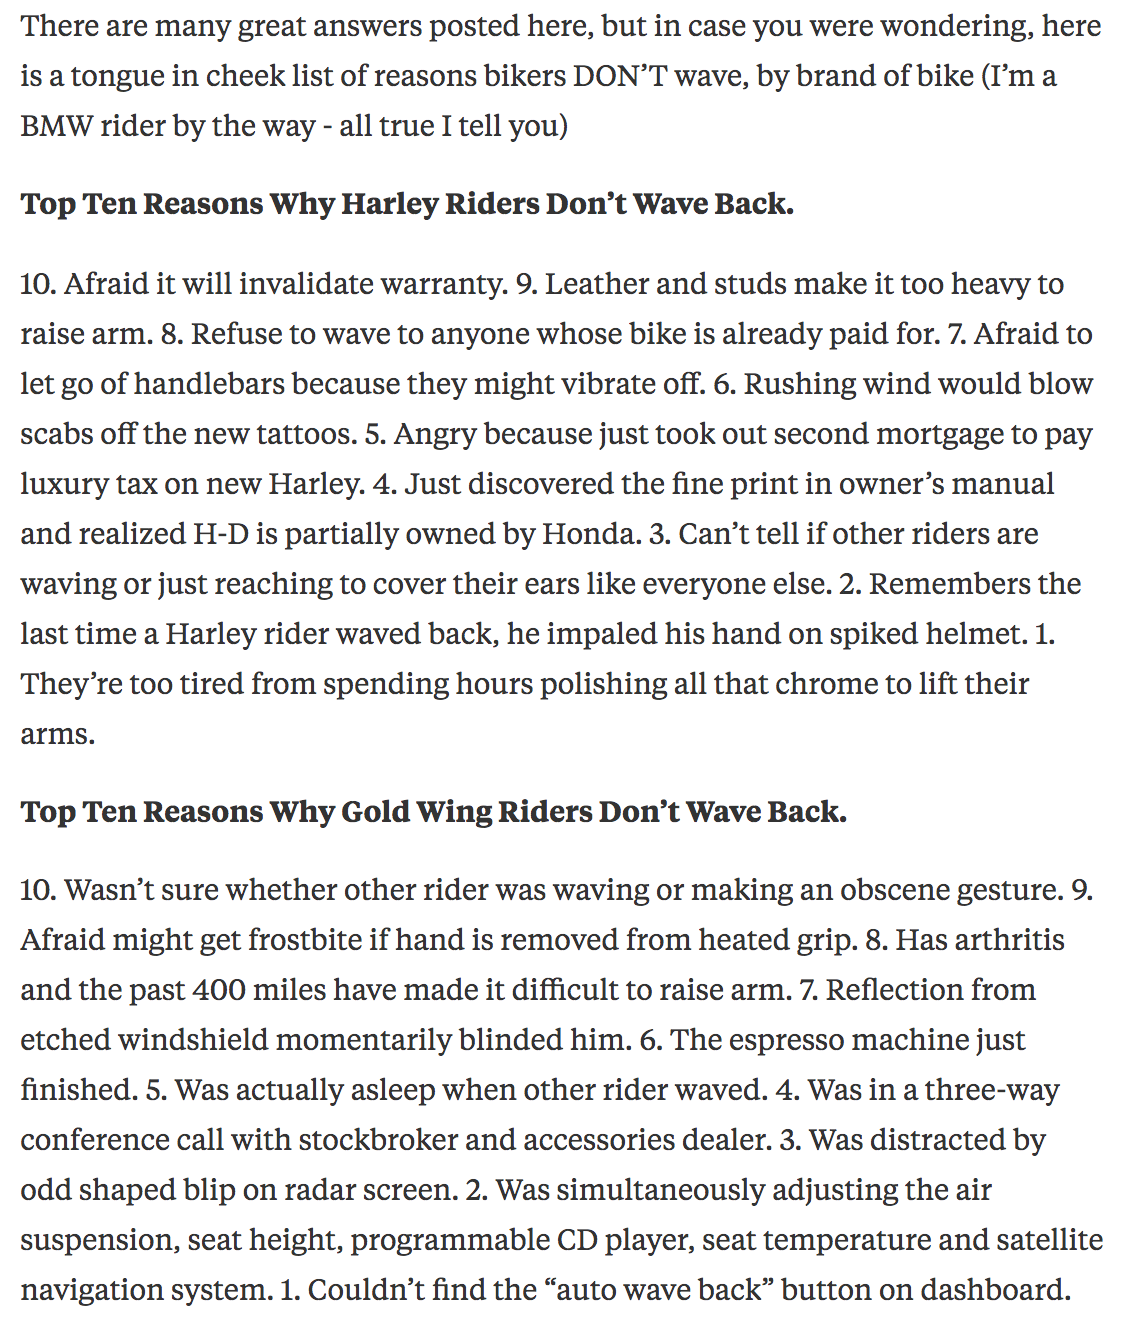
\includegraphics[scale=.5]{reasons.png}
\caption{Reasons motorcyclists don't wave back}
\end{figure}

As expected, the higher quality question returned higher quality answers that were in depth, on point and were written as clearly as possible to avoid any confusion to the reader. The low quality question received answers that were not serious, or not related. 

\section{Question 10.6}
\subsection {Question}
Find two examples of document filtering systems on the Web. How do they build a profile for your information need? Is the system static or adaptive?

\subsection{Answer}
\href{www.ebay.com}{Ebay} is an online shopping website that is used worldwide to purchase all sorts of goods from pencils to used car parts to baby clothes. It keeps track of what the user has been searching for and buying to create a profile of them. They use this profile to recommend more things to buy to the user as shown in the picture below. It is not as precise as I'd like but it still does a good enough job that I click the items that come up as recommended, probably once a month. It fails to distinguish brands. The bike I am looking for a fairing for is a Yamaha, yet it keeps showing me Suzuki fairings. 

\begin{figure}[h!]
\centering
\label{fig:ebay}
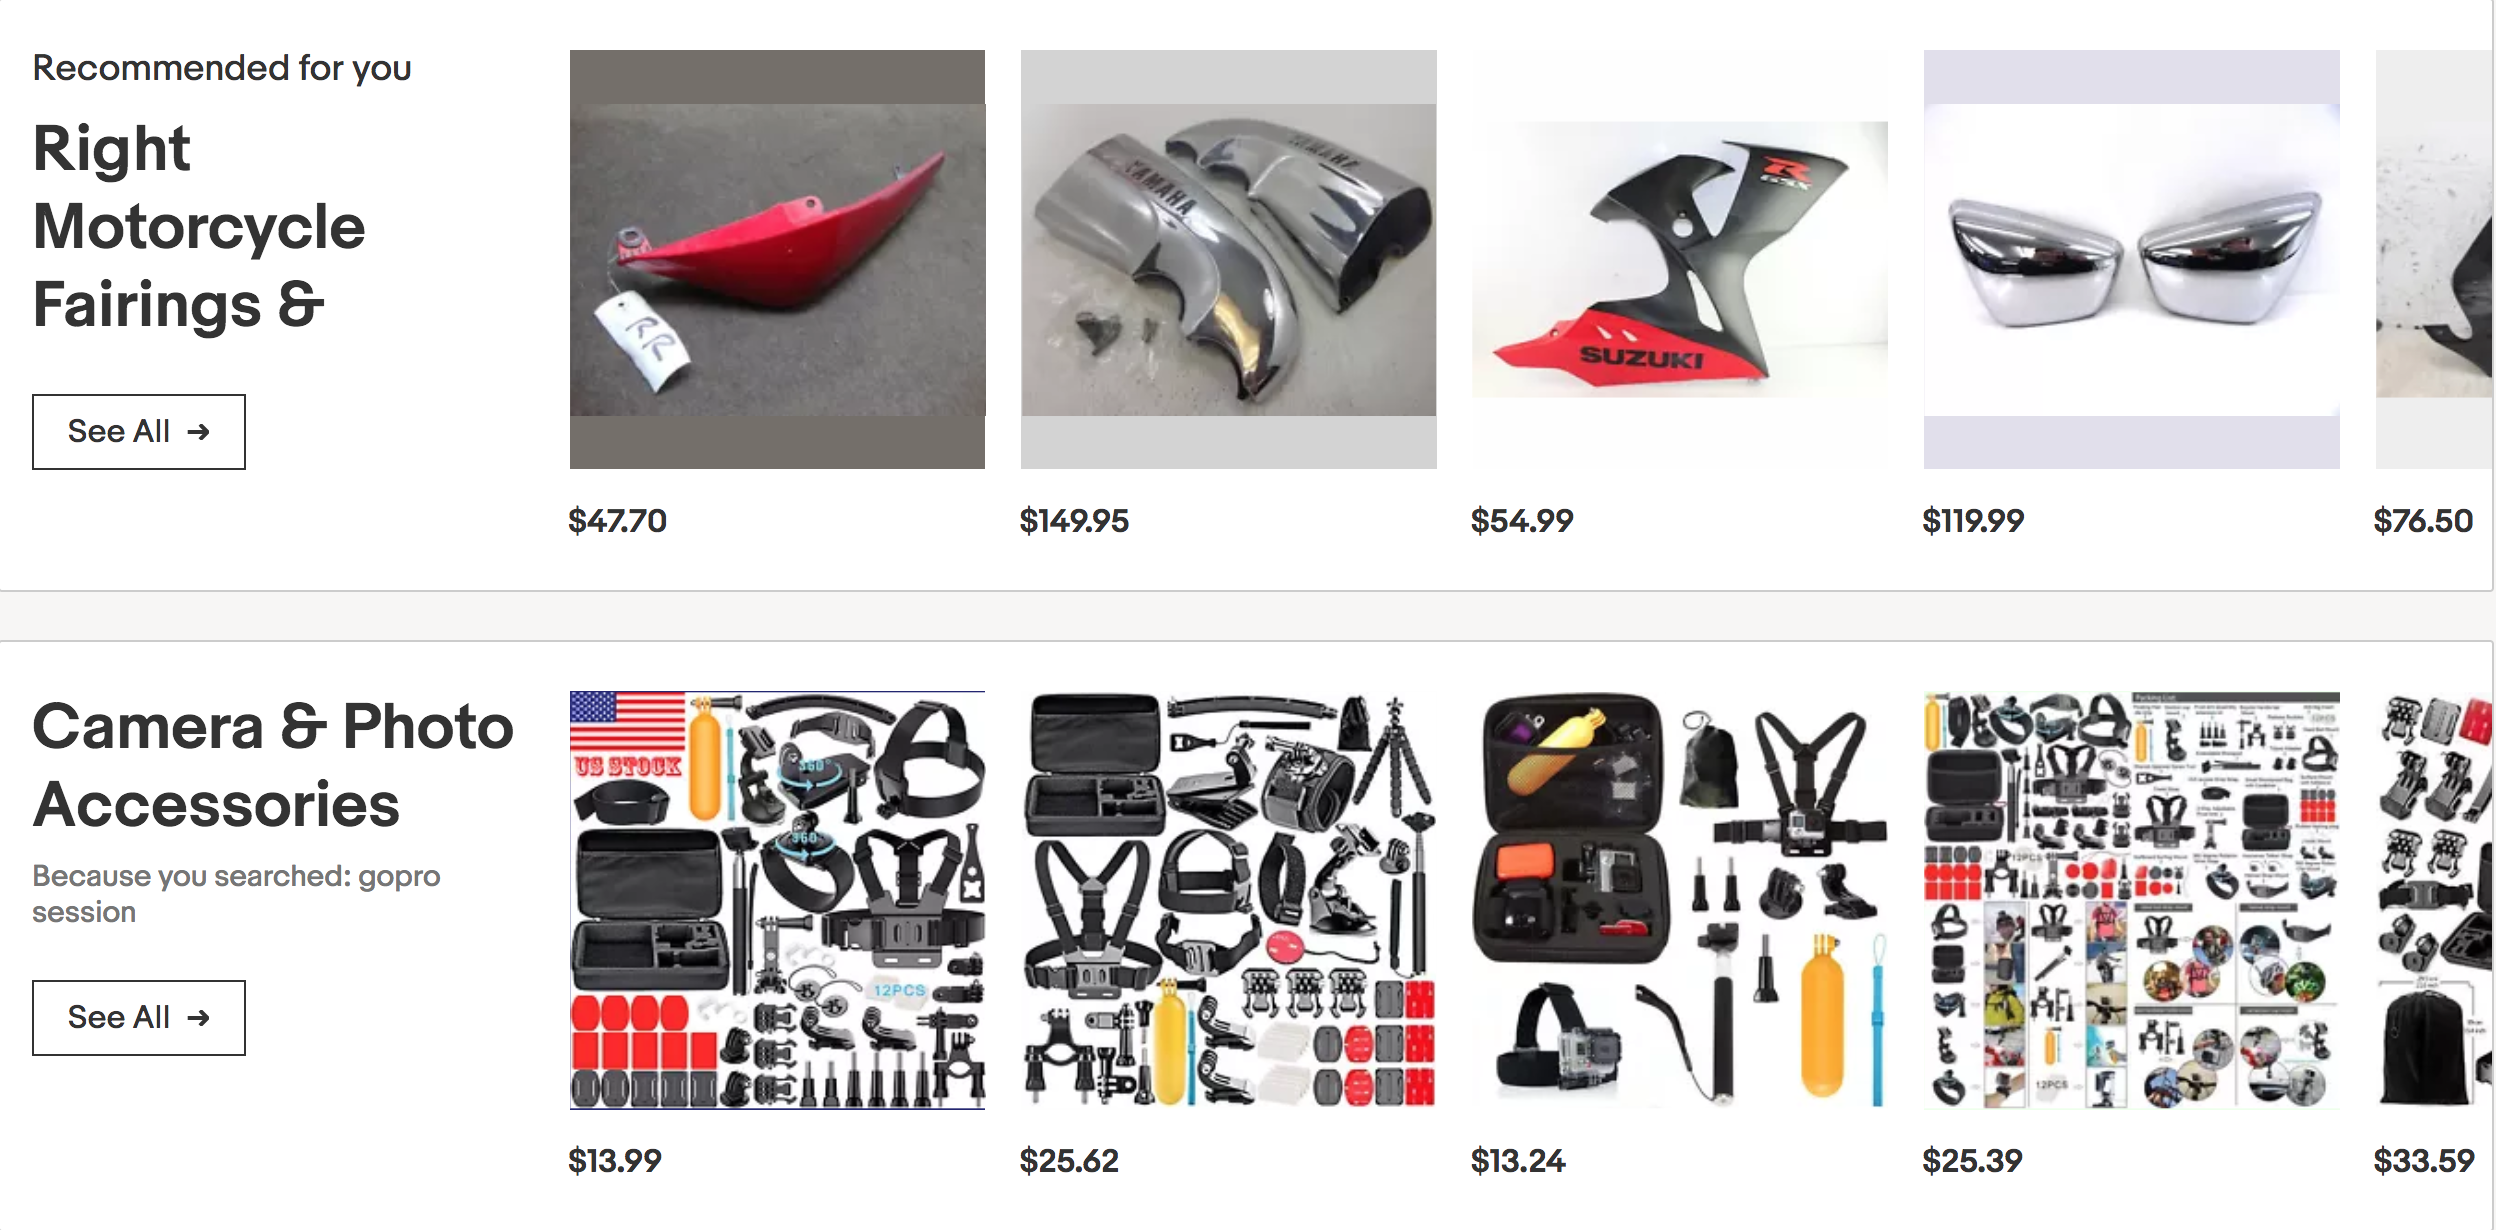
\includegraphics[scale=.5]{ebay.png}
\caption{Ebay recommended items}
\end{figure}

Classifying new items is simplified thanks to their very intensive categorization of the items. Users can create their ads by finding something similar for sale and simply clicking the button below the picture that says ``Have one to sell? Sell now''. This will fill out some fields for you depending on which ad you navigated from. But the main way to tell Ebay what you are selling is to use the categories listed when creating a new ad. This makes sure Ebay knows exactly what you are posting so it can decide to notify or not notify people looking for that item.

\begin{figure}[h!]
\centering
\label{fig:ebay-sell}
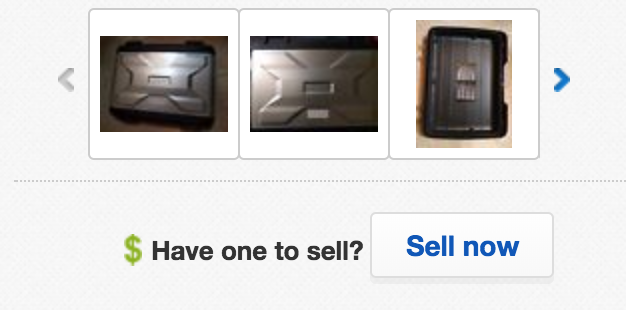
\includegraphics[scale=.5]{ebay-sell.png}
\caption{Ebay ``have one to sell'' button}
\end{figure}

\begin{figure}[h!]
\centering
\label{fig:ebay-category}
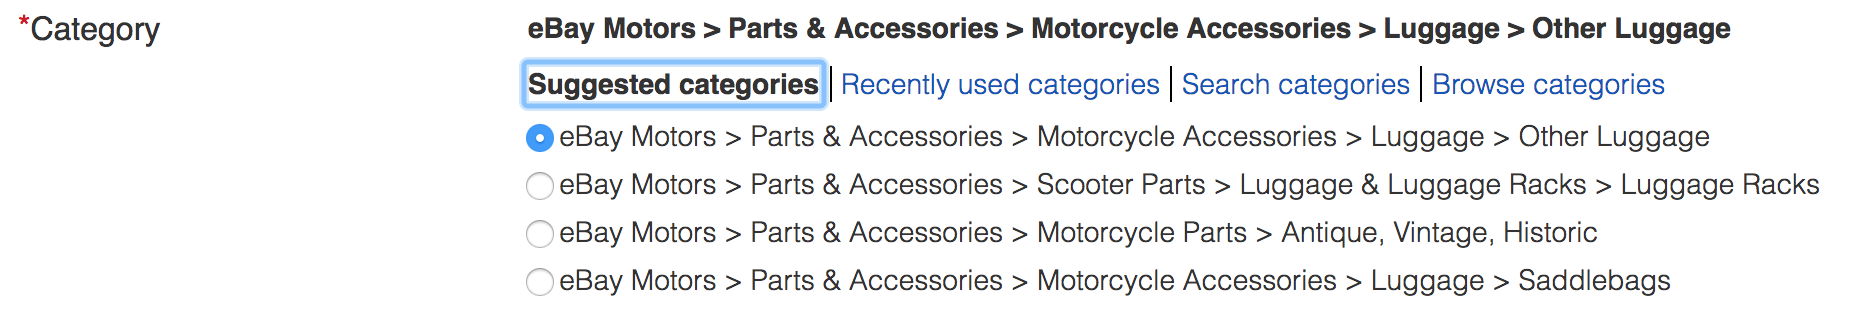
\includegraphics[scale=.5]{ebay-category.png}
\caption{Ebay category box}
\end{figure}

\href{www.youtube.com}{YouTube} is a video sharing platform owned by \href{www.google.com}{Google}. YouTube is a little different from your average e-commerce websites (Amazon, Ebay etc.). There are two different ways to view YouTube. First is the every day person's YouTube activity which is searching for a topic and watching videos about said topic. The second is following a content creator in which the user would watch videos made by the content creator even if he/she doesn't really care about the topic of that specific video. 

But the overall idea is the same in that each user will have a profile that consists of the types of videos they like to watch, the channels they have subscribed to and kind of videos they have skipped. For example it knows I like motorcycle videos. Therefore, it recommends motorcycle videos to me. It doesn't care as much about the specific topic of the video if I'm subscribed to the channel. YouTube is also biased thanks to millions of other viewers rating videos and making certain people more popular than others. So if someone popular on YouTube publishes a new video, it would appear in my home page even if I am not subscribed to that person. 

For new videos, it has an weighted evaluation function where it gives different properties of a video different weights. Since YouTube is a video sharing platform and videos aren't easy to crawl, it goes by the title, description, and tags. For example I make motorcycle videos on YouTube in Turkish. There are two types of viewers that watch my content. One is people who speak Turkish who are interested in motorcycles and the second is people who speak Turkish who are interested in life in the United States. After a year of doing it, I've noticed that YouTube gives a heavy weight to the video titles. Therefore, I try to include the word ``Amerika'' in my video titles to reach the latter type of audience. Basically trying to play tricks on the decision mechanism to boost my channel. Below is a screenshot of my YouTube Analytics page which shows what people searched for to find my channel. This is where I got the idea.

\begin{figure}[h!]
\centering
\label{fig:youtube-analytics}
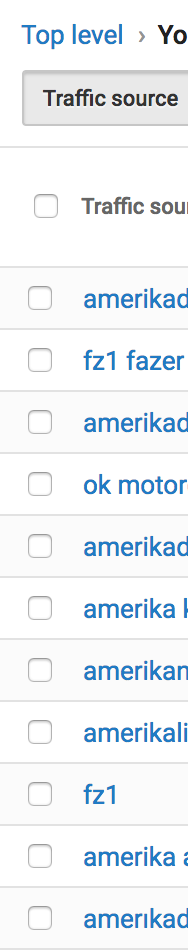
\includegraphics[scale=.5]{youtube-analytics.png}
\caption{YouTube traffic sources search results page}
\end{figure}

\section{Question 11.5}
\subsection {Question}
How many papers dealing with term dependency can you find in the SIGIR proceedings since 2000? List their citations.

\subsection{Answer}
Using \href{https://scholar.google.com/}{Google Scholar}'s advanced search tool, I was able to find all the papers that were published in SIGIR after 2000 that deal with term dependency. I used the advanced search tool because I am not very competent about using the specific symbols to tell Google what I want so I let the tool do it for me. Since the question said ``dealing with'' term dependency, I figured I'd include a couple variations of the search term so I searched for ``term dependency'' or ``term dependencies'' or ``term dependence''. I'm aware that stemming would probably take care of this for me but I didn't want to take chances. A screenshot of the search page is below. The list of the citations can be reached at \href{https://scholar.google.com/scholar?as_vis=0&q=term+dependencies+%7C+term+dependency+%7C+term+dependence+source:SIGIR&hl=en&as_sdt=2c47&as_ylo=2000}{this link}.

\begin{figure}[h!]
\centering
\label{fig:scholar-search}
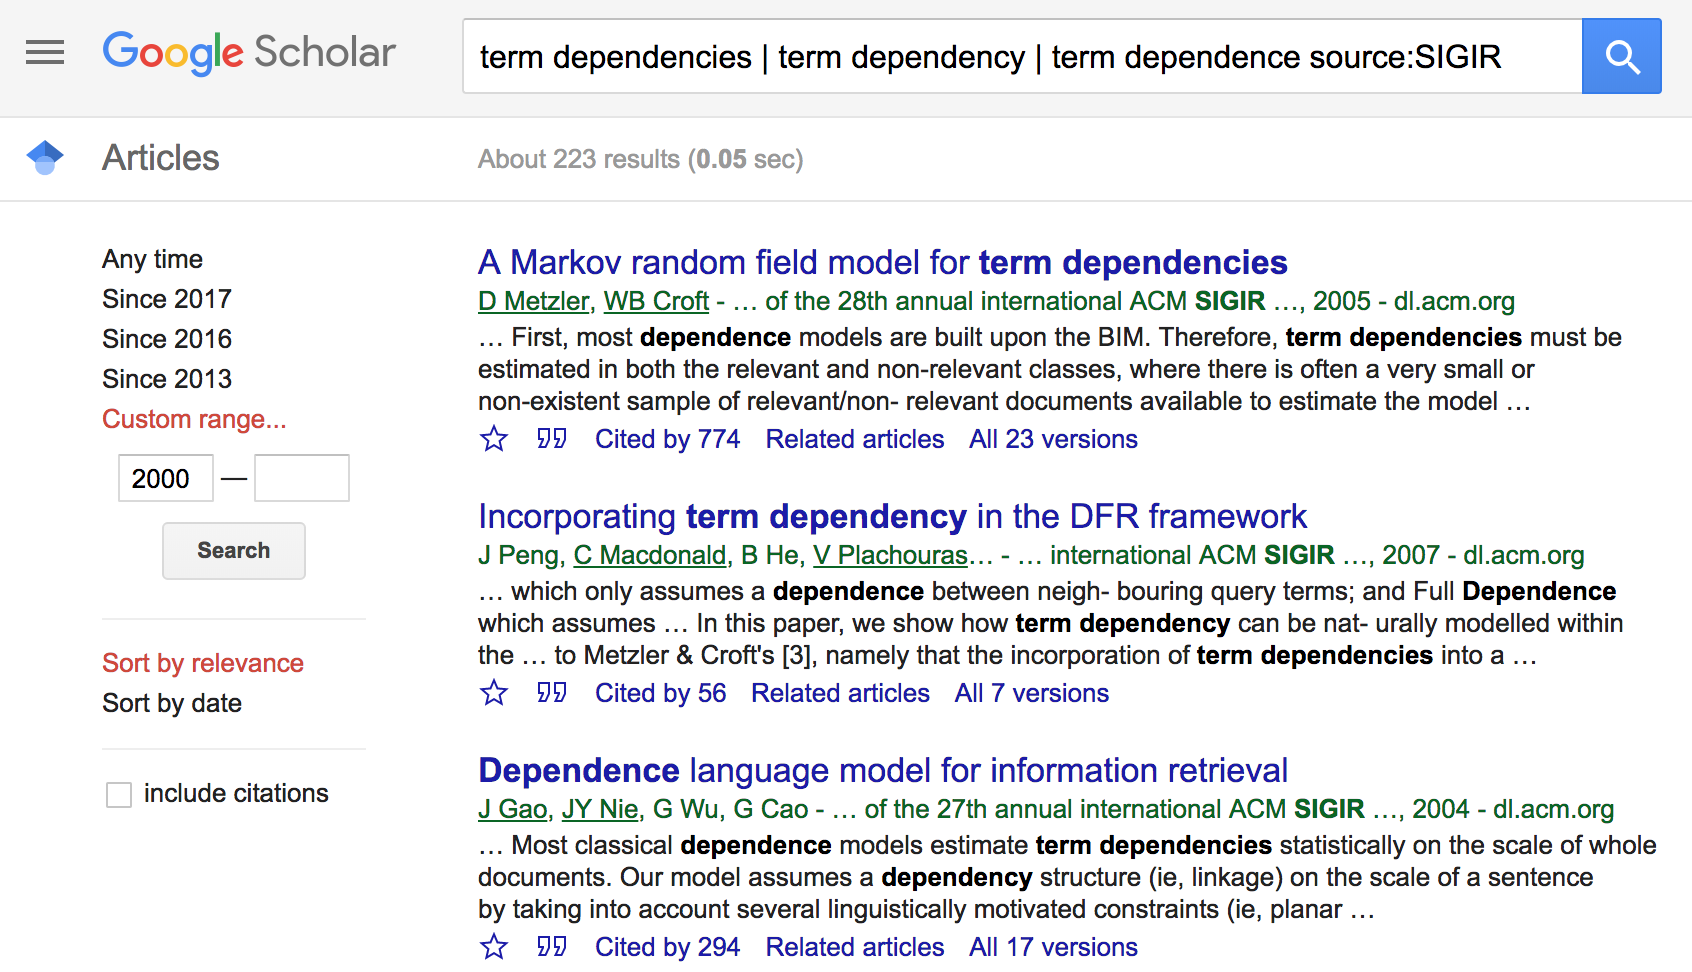
\includegraphics[scale=.5]{scholar-search.png}
\caption{Google Scholar search for SIGIR papers after 2000 dealing with term dependency}
\end{figure}

\section{Question 11.9}
\subsection{Question}
Find a demonstration of a question answering system running on the Web. Using a test set of questions, identify which types of questions work and which don’t on this system. Report effectiveness using MRR or another measure.

\subsection{Answer}
For this question I picked \href{http://start.csail.mit.edu/index.php}{MIT's START}. It is different than a search engine in that it tries to give you one, correct answer for your question instead of taking you to a list of pages that might have the answer you are looking for. But it is also similar to a search engine in that it will collect its answer from different resources. For example just entering ``Old Dominion University'' in the search bar and information from Wikipedia, and U.S. News. It also takes a little while (couple seconds) to present answers for your query.

It requires and produces English text so any other language will likely fail to produce results. It also fails to anwser questions that are subjective such as ``What is love?'', even though I receive a definition when I query ``love''. Unlike Google, it seems that it doesn't have a concept of popular query. When I query ``How does ABS work?'', I get information about the New Zealand rugby team All Blacks. I am expected to go over the other possible meanings of ABS and find the one I am looking for. So it is safe to say that abbreviations aren't the best way to go about using this system. 

So in order to calculate effectiveness, I will use the following sample queries:
\begin{itemize}
    \item How does clutch work
    \item What is black eyed pea (referring to the type of beans)
    \item How does ABS work
    \item The Killers (referring to the band)
    \item Ford
\end{itemize}

Since these are terms that have multiple meanings, for most cases, I received a list of possible meanings that seemed to be retrieved from Wikipedia. Below are screenshots of what I received for each query. In two of the five, I received what I was looking for immediately. This has to do with me trying to trick the system and querying things that have more than one meaning. Not many people search for black eyed pea, the bean.

\begin{figure}[h!]
\centering
\label{fig:start-clutch}
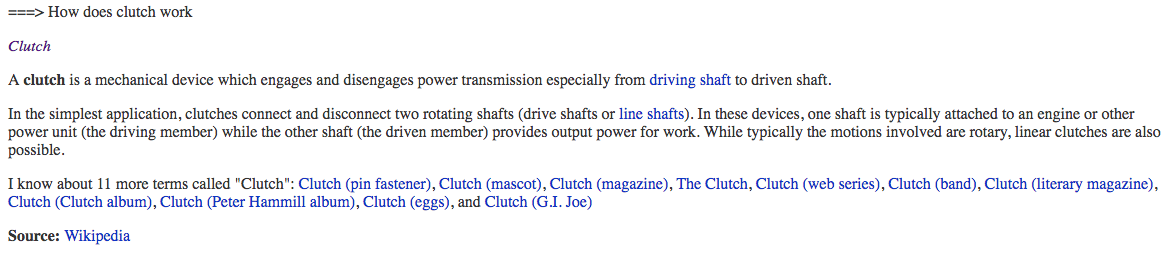
\includegraphics[scale=.5]{start-clutch.png}
\caption{START search results for clutch}
\end{figure}

\begin{figure}[h!]
\centering
\label{fig:start-black-eyed-pea}
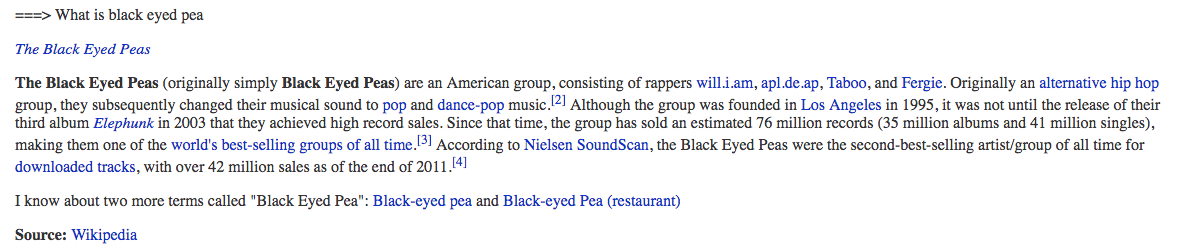
\includegraphics[scale=.5]{start-black-eyed-pea.png}
\caption{START search results for black eyed pea}
\end{figure}

\begin{figure}[h!]
\centering
\label{fig:start-abs}
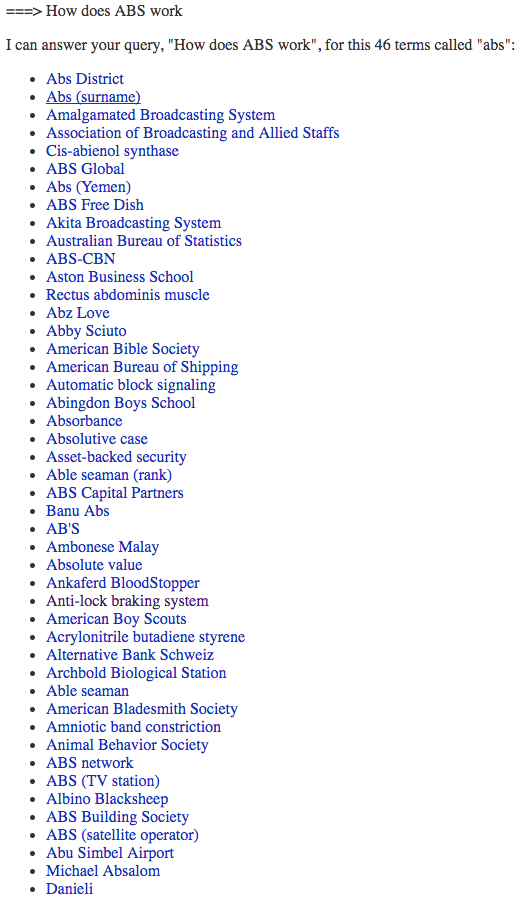
\includegraphics[scale=.5]{start-abs.png}
\caption{START search results for ABS}
\end{figure}

\begin{figure}[h!]
\centering
\label{fig:start-killers}
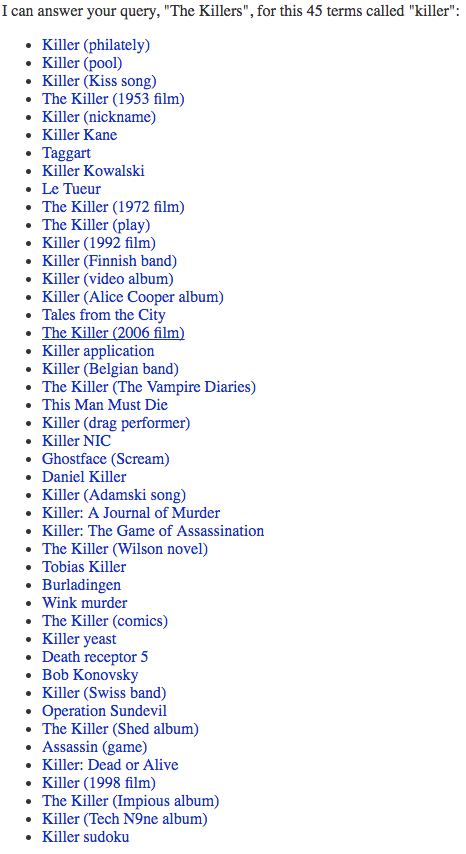
\includegraphics[scale=.5]{start-killers.png}
\caption{START search results for The Killers}
\end{figure}

\begin{figure}[h!]
\centering
\label{fig:start-ford}
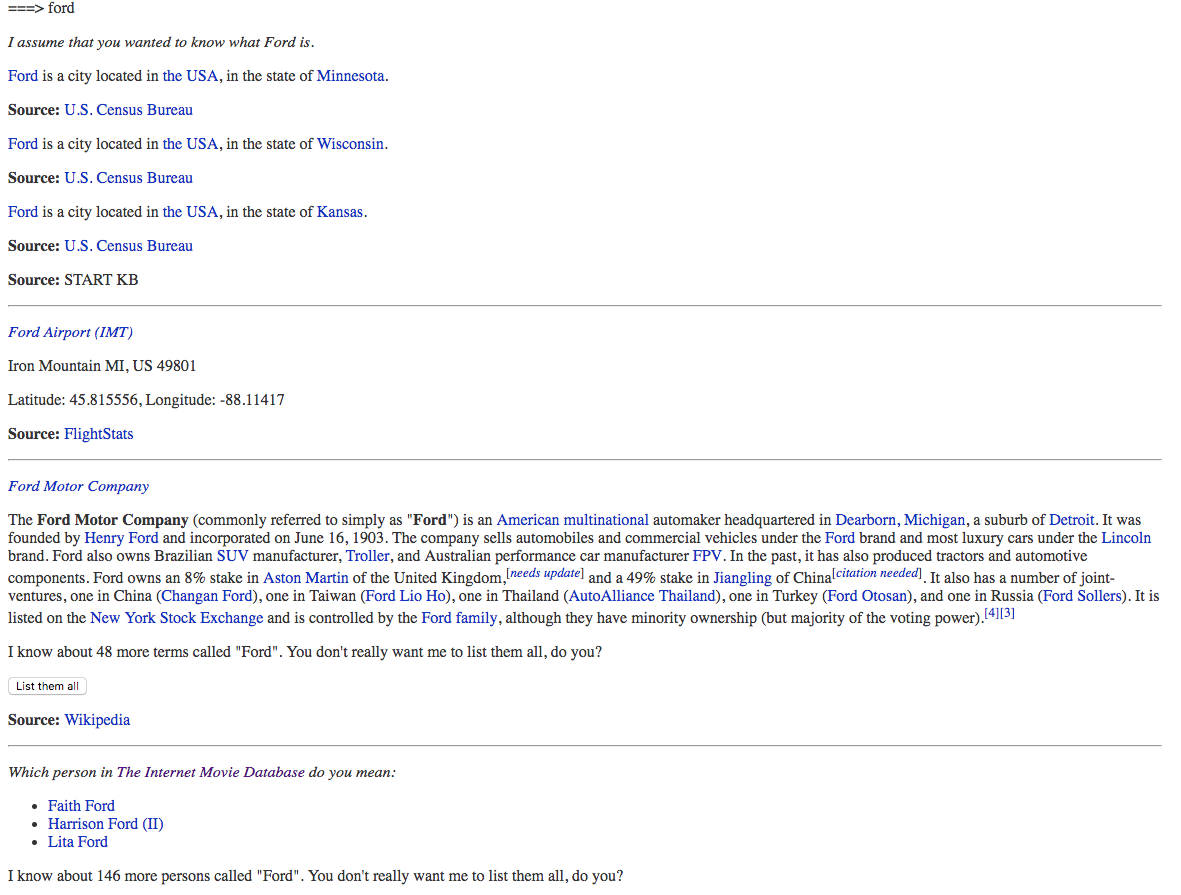
\includegraphics[scale=.5]{start-ford.png}
\caption{START search results for Ford}
\end{figure}

Overall, the mean reciprocal rank from these searches was: 
$\frac{1 + \frac{1}{2} + \frac{1}{31} + 0 + \frac{1}{5}}{5} = 0.346 $

\section{Question 11.11}
\subsection{Question}
Look at a sample of images or videos that have been tagged by users and separate the tags into three groups: those you think could eventually be done automatically by image processing and object recognition, those you think would
not be possible to derive by image processing, and spam. Also decide which of the tags should be most useful for queries related to those images. Summarize your findings.

\subsection{Answer}
I chose the popular image based social media \href{www.instagram.com}{Instagram} to answer this question. Users upload their images to Instagram and add tags using the \# sign. Tags are short phrases that explain the image uploaded. Many users use the tags to reach a wider audience. Instagram works on likes and follows. A picture with more likes will likely be shown to more people and follower counts are considered for marketing purposes. That's why spam tags such as \#likeforlike and \#likeforfollow are very common on accounts that are trying to advance in the ``Instagram world''. While some tags can be generated automatically, some aren't easy to identify via image processing and other techniques. Tags such as \#smile can be generated by image processing. But it would be hard to automatically generate tags that convey emotion such as \#happy which returns 407 million results. 

A sample of these tags can be seen in the screenshots below. Users try to use as many tags to reach as many people as possible. The second picture belongs to an account called \href{www.instagram.com/onherbike}{onherbike}. It is the Instagram account of a motorcycle travel blogger. She uses Instagram tags to build her audience which she needs to be able to do her travels. She is sponsored by many companies including \href{www.bmw-motorrad.com/com/en/}{BMW Motorcycles} who probably require her to use these tags on her pictures. The third picture is a screenshot of many spam tags. The content of the picture is not very relevant in this case as the tags don't reflect anything in the picture. They are simply used to lure people.

\begin{figure}[h!]
\centering
\label{fig:insta-tag1}

\includegraphics[scale=.5]{insta-tag1.png}
\caption{More tags = More people}
\end{figure}

This user is trying to reach an audience that is interested in motorcycles, especially cafe racers. Even though it is hard to tell much about the motorcycle from this picture, it is generally visually pleasing, so maybe more general tags such as \#adventure, \#reflection would have increased the range (how many people it reaches) of this post. Longer tags are usually not preferred as it kind of beats the purpose of tags so the tags that benefited this post the most are likely the shorter ones such as \#motorcycle, \#caferacer and \#biker.

\begin{figure}[h!]
\centering
\label{fig:insta-tag2}

\includegraphics[scale=.5]{insta-tag2.png}
\caption{Users use tags to build up an audience to promote their product}
\end{figure}

The user that posted this picture is sponsored by BMW so it is normal to see all the BMW tags in all her pictures. Location tags such as \#istanbul are very popular which has likely benefited this post more than the others. \#makelifearide doesn't seem like an optimal tag as it doesn't convey much information in itself. Upon clicking on it, I noticed that this tag is mostly used by BMW motorcycle riders who already use all the other similar tags. So most of the tags that are used in this post have the same audience and therefore can be ignored. \#motorcycle, just like the first example is a useful tag that will draw people. \#spiritofGS, probably not that important for this post.

\begin{figure}[h!]
\centering
\label{fig:insta-spam}
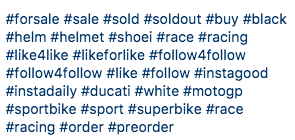
\includegraphics[scale=.5]{insta-spam.png}
\caption{Sample spam tags}
\end{figure}

\section{Question Extra Credit}
\subsection{Question}
Work through the "Inductive SVM" example, discuss in detail the steps and resulting output

\subsection{Methodology}
Using the SVM\textsuperscript{light} which can be found \href{http://www.cs.cornell.edu/people/tj/svm_light/}{here}, I was able to run the example and receive the results. 

\subsection{Results}
Below is a screenshot of running SVM\textsuperscript{light} on the provided dataset as per the instructions.

\begin{figure}[h!]
\centering
\label{fig:svm_light}
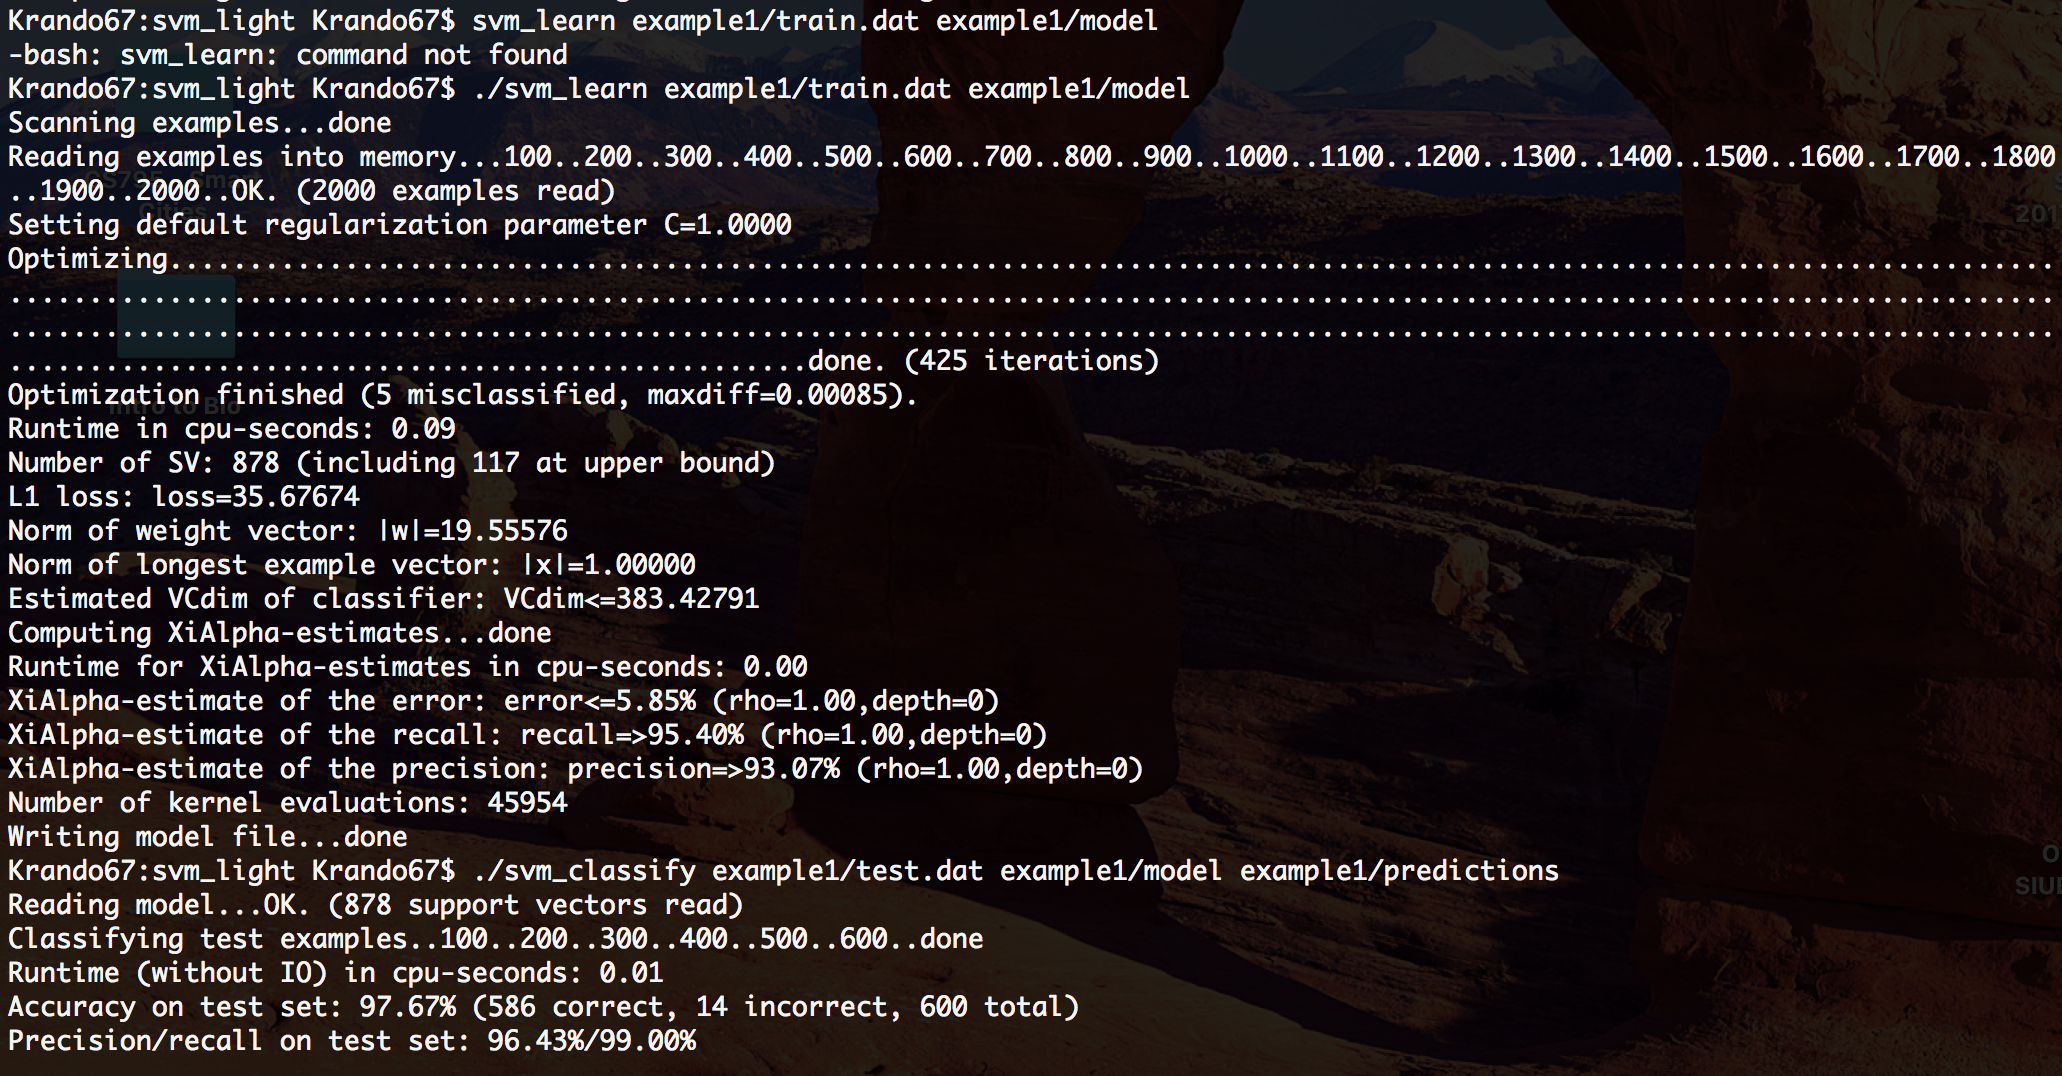
\includegraphics[scale=.5]{svm_light_results.png}
\caption{Results from SVM\textsuperscript{light}}
\end{figure}

The program provided the scores of 96.43\% for precision and 99\% for recall. These are expected results since the example is created by the author of the program. The \texttt{svm\_learn} executable goes through the training data and creates the support vectors, provides XiAlpha estimates and creates a model file to be used by the \texttt{svm\_classify} executable. 

The \texttt{svm\_classify} executable uses the model file created by \texttt{svm\_learn} to try to classify the test data into the classifications using the support vectors and provides the performance values which are very high for this set of test data. This means that the training data is very high quality. 

% \clearpage
% \begin{thebibliography}{9}
% \bibitem{classtext}
%     Croft, William Bruce, et al. \textit{Search Engines: Information Retrieval in Practice}. Pearson, 2010.
% \end{thebibliography}
\end{document}